\scanpage{98}
\diagram{\begin{tikzcd}[ampersand replacement=\&,column sep=0pt,row sep=0pt]
{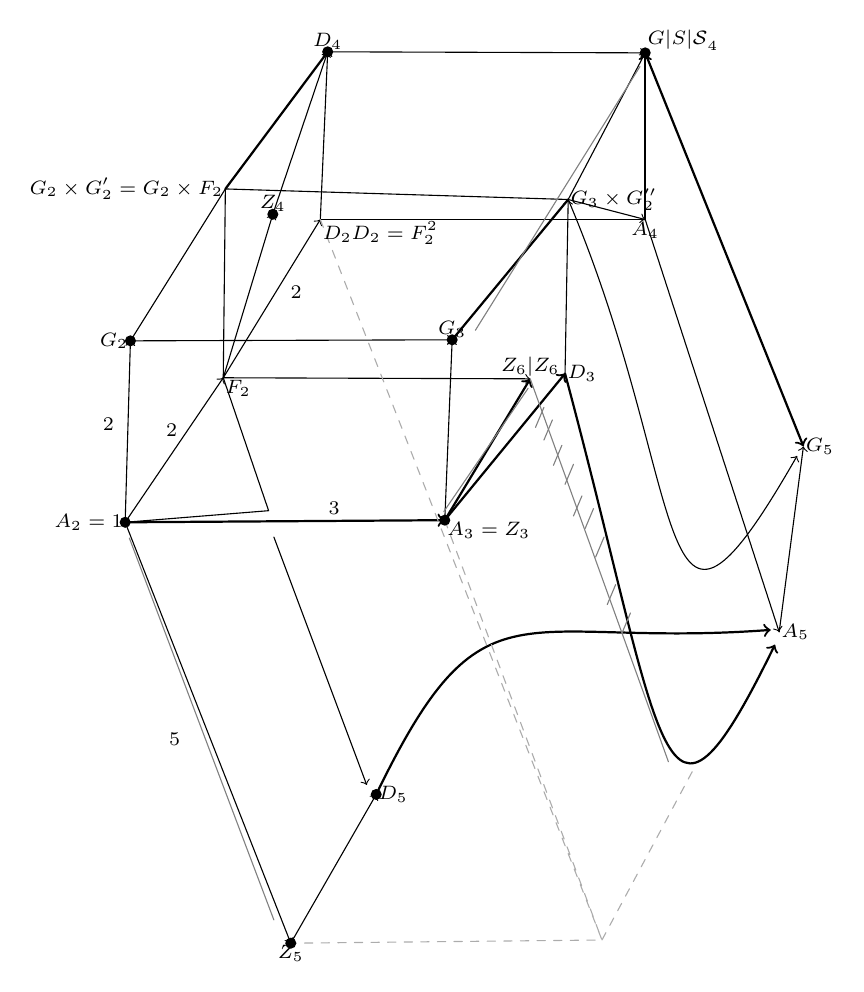
\begin{tikzpicture}[x=.0134cm,y=-.0134cm,line cap=round,line join=round,baseline=(current bounding box.center)]
\coordinate (D4) at (327,133);
\coordinate (G4) at (628,134);
\coordinate (V) at (230,263);
\coordinate (Z4) at (275,287);
\coordinate (D2) at (320,292);
\coordinate (D6) at (555,273);
\coordinate (A4) at (628,292);
\coordinate (G2) at (140,407);
\coordinate (F2) at (228,442);
\coordinate (G3) at (445,406);
\coordinate (Z6) at (519,443);
\coordinate (D3) at (552,438);
\coordinate (G5) at (778,507);
\coordinate (A2) at (135,579);
\coordinate (A3) at (438,577);
\coordinate (A5) at (755,683);
\coordinate (D5) at (373,837);
\coordinate (Z5) at (292,978);
\draw[->] (D4)--(G4);
\draw[-,thick] (V)--(D4);
\draw[->] (Z4)--(D4);
\draw[->] (D2)--(D4);
\draw[thin] (V)--(D6);
\draw[thin] (D2)--(A4);
\draw[->] (D6)--(A4);
\draw[->,thick] (A4)--(G4);
\draw[->,thick] (G4)--(G5);
\draw[thin] (G2)--(V);
\draw[->] (G2)--(G3);
\draw[thin] (V)--(F2);
\draw[->] (F2)--(Z4);
\draw[->] (F2)--(D2);
\draw[-,thick] (G3)--(D6);
\draw[->] (D6)--(G4);
\draw[->] (A3)--(G3);
\draw[->] (A2)--(G2);
\draw[->] (A2)--(F2);
\draw[->,thick] (A2)--(A3);
\draw[->] (F2)--(Z6);
\draw[->,thick] (A3)--(Z6);
\draw[->,thick] (A3)--(D3);
\draw[->] (D3)--(D6);
\draw[->] (A5)--(G5);
\draw[->] (A4)--(A5);
\draw[->] (A2)--(Z5);
\draw[->] (Z5)--(D5);
\draw[->] (276,593)--(364,828);
\draw (F2)--(271,568)--(A2);
\draw[->,thick] (D5) .. controls (475,626) and (506,699) .. (747,681);
\draw[->,thick] (D3) .. controls (648,796) and (642,918) .. (751,695);
\draw[->] (D6) .. controls (673,551) and (633,759) .. (772,516);
\draw[gray!65,dashed] (D2)--(587,975)--(Z5) (A3)--(587,975)--(676,809);
\draw[gray] (Z6)--(650,806) (139,594)--(276,956) (467,397)--(623,147) (437,569)--(517,452);
\foreach \a/\b in {4/0,12/4,21/12,32/18,40/28,51/32,61/41,72/56,86/65}{\draw[gray,thin] (528+\a,470+3*\b)--(520+\a,489+3*\b);}
\foreach \i in {A2,A3,G3,G2,Z4,D4,G4,D5,Z5}{\fill (\i) circle (2pt);}
\node[anchor=south,inner sep=.7pt,font=\scriptsize] at (D4) {$D_4$};
\node[anchor=south west,inner sep=.7pt,font=\scriptsize] at (G4) {${\unsure{G|\mathfrak S|\mathcal S}}_4$};
\node[anchor=east,inner sep=.7pt,font=\scriptsize] at (V) {$G_2\times G'_2=G_2\times\mathbb F_2$};
\node[anchor=south,inner sep=.7pt,font=\scriptsize] at (Z4) {$Z_4$};
\node[anchor=north west,inner sep=.7pt,font=\scriptsize] at (D2) {$\deleted{\unsure{D_2}}D_2=F_2^2$};
\node[anchor=west,inner sep=.7pt,font=\scriptsize] at (D6) {$G_3\times G''_2$};
\node[anchor=north,inner sep=.7pt,font=\scriptsize] at (A4) {$A_4$};
\node[anchor=east,inner sep=.7pt,font=\scriptsize] at (G2) {$G_2$};
\node[anchor=north west,inner sep=.7pt,font=\scriptsize] at (F2) {$F_2$};
\node[anchor=south,inner sep=.7pt,font=\scriptsize] at (G3) {$G_3$};
\node[anchor=south,inner sep=.7pt,font=\scriptsize] at (Z6) {$\deleted{\unsure{Z_6|\mathbb Z_6}}$};
\node[anchor=west,inner sep=.7pt,font=\scriptsize] at (D3) {$D_3$};
\node[anchor=west,inner sep=.7pt,font=\scriptsize] at (G5) {$G_5$};
\node[anchor=east,inner sep=.7pt,font=\scriptsize] at (A2) {$A_2=1$};
\node[anchor=north west,inner sep=.7pt,font=\scriptsize] at (A3) {$A_3=Z_3$};
\node[anchor=west,inner sep=.7pt,font=\scriptsize] at (A5) {$A_5$};
\node[anchor=west,inner sep=.7pt,font=\scriptsize] at (D5) {$D_5$};
\node[anchor=north,inner sep=.7pt,font=\scriptsize] at (Z5) {$Z_5$};
\node[anchor=center,inner sep=.7pt,font=\scriptsize] at (119,486) {$2$};
\node[anchor=center,inner sep=.7pt,font=\scriptsize] at (179,492) {$2$};
\node[anchor=center,inner sep=.7pt,font=\scriptsize] at (297,361) {$2$};
\node[anchor=center,inner sep=.7pt,font=\scriptsize] at (333,566) {$3$};
\node[anchor=center,inner sep=.7pt,font=\scriptsize] at (182,785) {$5$};
\end{tikzpicture}}
\end{tikzcd}}
les \deleted{\unsure{17}}18 \inserted{classes de} sous-groupes de $G_5$

\margin{\tikz[baseline=(q.base)]{\node[align=center] (q) {dont\\ 9 abéliens}; \draw (q.center) ellipse (3em and 1.8em);}}
\[
\begin{aligned}
[9]\ &\text{classes de ss-gpes de }A_5\\
11\ &\text{classes de ss-gpes de }G_4\\
5\ &\text{classes de ss-gpes de }A_4\\
4\ &\text{classes de ss gpes de }G_3\\
7\ &\text{classes de ss-gpes de }D_4\\
10\ &\rule{4.8em}{.5pt}\quad\widetilde G_3\\[-3pt]
&\quad\text{\uuline{\hspace{2.0em}}}
\end{aligned}
\]
\unsure{1}
\diagram{\begin{tikzcd}[ampersand replacement=\&,column sep=0pt,row sep=0pt]
{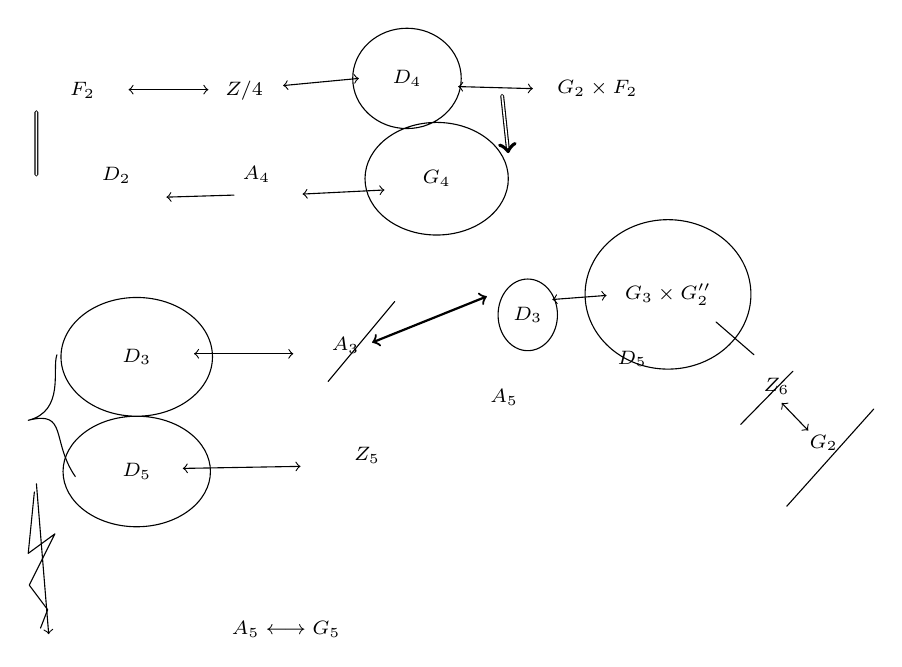
\begin{tikzpicture}[x=.013cm,y=-.013cm,line cap=round,line join=round,baseline=(current bounding box.center)]
\coordinate (f) at (95,1268);
\coordinate (z) at (253,1268);
\coordinate (d) at (412,1256);
\coordinate (v) at (598,1266);
\coordinate (p) at (128,1351);
\coordinate (a) at (265,1350);
\coordinate (s) at (441,1354);
\coordinate (D) at (148,1528);
\coordinate (A) at (352,1517);
\coordinate (Dprime) at (530,1487);
\coordinate (vprime) at (667,1467);
\coordinate (z6) at (773,1557);
\coordinate (g2) at (819,1612);
\coordinate (d5) at (148,1640);
\coordinate (z5) at (373,1624);
\draw[<->] (140,1267)--(218,1267);
\draw[<->] (291,1263)--(365,1256);
\draw[<->] (462,1264)--(535,1266);
\draw[->,double] (50,1289)--(50,1350) (505,1273)--(511,1329);
\draw[<-] (177,1372)--(243,1370);
\draw[<->] (310,1369)--(390,1365);
\draw (d) ellipse (53 and 49) (s) ellipse (70 and 55);
\draw[<->] (204,1525)--(301,1525);
\draw[<->,thick] (378,1514)--(490,1469);
\draw[<->] (554,1472)--(607,1468);
\draw[<->] (714,1494)--(751,1526) (778,1573)--(804,1600);
\draw[<->] (193,1637)--(308,1635);
\draw (D) ellipse (74 and 58) (d5) ellipse (72 and 54) (Dprime) ellipse (29 and 35) (vprime) ellipse (81 and 73);
\draw[thin] (335,1552)--(400,1474) (738,1594)--(789,1542) (783,1674)--(868,1579);
\draw (70,1526)..controls(65,1540)and(78,1581)..(42,1590)..controls(81,1580)and(64,1610)..(88,1645);
\draw[->] (50,1652)--(62,1799);
\draw[thin] (48,1660)--(42,1720)--(68,1701)--(43,1751)--(61,1775)--(54,1793);
\node[anchor=center,inner sep=.7pt,font=\scriptsize] at (f) {$F_2$};
\node[anchor=center,inner sep=.7pt,font=\scriptsize] at (z) {$\mathbb Z/4$};
\node[anchor=center,inner sep=.7pt,font=\scriptsize] at (d) {$D_4$};
\node[anchor=center,inner sep=.7pt,font=\scriptsize] at (v) {$G_2\times F_2$};
\node[anchor=center,inner sep=.7pt,font=\scriptsize] at (p) {$D_2$};
\node[anchor=center,inner sep=.7pt,font=\scriptsize] at (a) {$A_4$};
\node[anchor=center,inner sep=.7pt,font=\scriptsize] at (s) {$G_4$};
\node[anchor=center,inner sep=.7pt,font=\scriptsize] at (D) {$D_3$};
\node[anchor=center,inner sep=.7pt,font=\scriptsize] at (A) {$A_3$};
\node[anchor=center,inner sep=.7pt,font=\scriptsize] at (Dprime) {$D_3$};
\node[anchor=center,inner sep=.7pt,font=\scriptsize] at (vprime) {$G_3\times G''_2$};
\node[anchor=center,inner sep=.7pt,font=\scriptsize] at (z6) {$Z_6$};
\node[anchor=center,inner sep=.7pt,font=\scriptsize] at (g2) {$G_2$};
\node[anchor=center,inner sep=.7pt,font=\scriptsize] at (d5) {$D_5$};
\node[anchor=center,inner sep=.7pt,font=\scriptsize] at (z5) {$Z_5$};
\node[anchor=center,inner sep=.7pt,font=\scriptsize] at (507,1568) {$\deleted{\unsure{A_5}}$};
\node[anchor=center,inner sep=.7pt,font=\scriptsize] at (632,1530) {$\deleted{\unsure{D_5}}$};
\node[anchor=center,inner sep=.7pt,font=\scriptsize] at (294,1794) {$\deleted{\unsure{A_5\longleftrightarrow G_5}}$};
\end{tikzpicture}}
\end{tikzcd}}
\[
\left\{\begin{aligned}
F_2&=\mathfrak z(D_4)=\mathfrak z(D_4,G_4)\\
D_4&=N(F_2\unsure{,|;}G_4)\\
F_2&=2\cdot Z_4={}_2(Z_4)\\
D_4&=N(Z_4,G_4)\\
Z_4&=\text{gpe engendré par \unsure{l'un des|n'importe les|n'importe}}\\
 &\quad\text{\unsure{quels|quelconque|quel} des 2 \unsure{élts|élt|él.} d'ordre}\\
 &\quad 4\ \text{de }D_4
\end{aligned}\right.
\]
\[
\begin{aligned}
G_{\unsure{4|5}}&=N(D_2^{\unsure{2|*}},G_5)\\
D_2^{\unsure{2}}\!&=\text{seul sous-gpe invariant}\\
 &\quad\text{de }G_4\text{ d'indice }6
\end{aligned}
\]
\figure{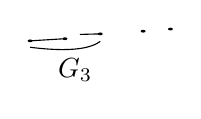
\begin{tikzpicture}[scale=.68]
\foreach \x/\y in {0/0,.65/.04,1.31/.13,2.11/.18,2.62/.22}{\fill (\x,\y) ellipse (.046 and .026);}
\draw (0,0)--(.65,.04) (.93,.12)--(1.31,.13);
\draw (0,-.12)..controls(.8,-.22)and(1.15,-.13)..(1.31,-.01);
\node[below] at (.84,-.14) {$G_3$};
\end{tikzpicture}}
\diagram{\begin{tikzcd}[ampersand replacement=\&]
G_{3}\arrow[d,dash]\\ A_{\unsure{2|6|3}}
\end{tikzcd}}
\diagram{\begin{tikzcd}[ampersand replacement=\&]
G_2\arrow[r,dash]\arrow[d,dash]\&G_3\arrow[r,dash]\arrow[d,dash]\&
G^{\unsure{1|'}}_{\unsure{3|2}}\times G'_{\unsure{3|2}}\arrow[d,dash]\\
{}\arrow[r,dash]\&A_3\arrow[r,dash]\&D_3
\end{tikzcd}}
% archive sheet number: 97
